\chapter{Results}
This chapter presents the evaluation of our LSTM model by comparing its performance to simpler heuristic approaches and the Majority Class Prediction (MCP) baseline. The comparison focuses on metrics such as accuracy, precision, recall, F1-scores, ROC-AUC, and PR-AUC, providing insights into the model's ability to classify DAOs as abandoned (inactive) or operating (active).

The LSTM model achieved an accuracy of 75\% on the test dataset. It effectively identified abandoned DAOs, with a precision of 0.77, recall of 0.83, and an F1-score of 0.80. For operating DAOs, the model achieved a precision of 0.71, recall of 0.63, and an F1-score of 0.67. These results indicate that the model excels in identifying inactive projects, though its performance is lower for active ones. The macro and weighted averages, with F1-scores of 0.73 and 0.74 respectively, confirm its balanced capability across both classes (see Table \ref{tab:lstm_res} of the Appendix).

In comparison, heuristic models displayed varying levels of effectiveness. The Twitter Follower Heuristic (TFH), which classifies DAOs based on upward trends in follower counts, achieved an accuracy of 64\% and a weighted F1-score of 0.64. It performed well for abandoned DAOs, achieving a precision of 0.73 and an F1-score of 0.62, but its recall of 0.54 indicates difficulty in capturing true positives. For operating DAOs, it achieved a precision of 0.58, recall of 0.76, and an F1-score of 0.66, suggesting a better ability to identify active projects despite some false positives.
The Price Trend Heuristic (PTH), which uses upward price movements as a signal for activity, achieved an accuracy of 68\% and a weighted F1-score of 0.65. It excelled in precision for operating DAOs, achieving 0.76, but struggled with recall (0.32), resulting in an F1-score of 0.45. For abandoned DAOs, the model achieved a precision of 0.67, recall of 0.93, and an F1-score of 0.78, reflecting a bias toward predicting inactivity over activity.
The Development Activity Heuristic (DAH), which classifies DAOs as active based on recent development activity, achieved 73\% accuracy and a weighted F1-score of 0.73, the highest among the heuristic methods. For operating DAOs, it achieved a precision of 0.77, recall of 0.66, and an F1-score of 0.71, reflecting a good balance between capturing true positives and minimizing false positives. For abandoned DAOs, it achieved a precision of 0.70, recall of 0.81, and an F1-score of 0.75, demonstrating consistent performance across both classes.
These results, summarized in Table \ref{tab:mlmodel_comparison}, show a slight superiority of the LSTM model, particularly in identifying abandoned DAOs, while heuristic approaches provide varying levels of trade-offs between precision and recall.

\begin{table}[h]
    \centering
    \caption{Comparison of Model Performance.}
    \begin{adjustbox}{max width=\textwidth}
        \begin{tabular}{llcccc}
            \toprule
            \textbf{Model} & \textbf{Classes} & \textbf{Precision} & \textbf{Recall} & \textbf{F1-Score} & \textbf{Accuracy} \\
            \midrule
            \multirow{2}{*}{Twitter Trend (TFH)} & Abandoned  & 0.73 & 0.54 & 0.62 & \multirow{2}{*}{0.64} \\ & Operating  & 0.58 & 0.76 & 0.66 &                     \\
            \midrule
            \multirow{2}{*}{Price Trend (PTH)} & Abandoned  & 0.67 & 0.93 & 0.78 & \multirow{2}{*}{0.68} \\ & Operating  & 0.76 & 0.32 & 0.45 &                     \\
            \midrule
            \multirow{2}{*}{Dev Activity (DAH)} & Abandoned  & 0.70 & 0.81 & 0.75 & \multirow{2}{*}{0.73} \\ & Operating  & 0.77 & 0.66 & 0.71 &                     \\
            \midrule
            \multirow{2}{*}{LSTM Model} & Abandoned  & 0.77 & 0.83 & 0.80 & \multirow{2}{*}{0.75} \\ & Operating  & 0.71 & 0.63 & 0.67 &                     \\
            \bottomrule
        \end{tabular}
    \end{adjustbox}
    \label{tab:mlmodel_comparison}
\end{table}

The performance of the LSTM model was further benchmarked against the Majority Class Prediction (MCP) baseline, which always predicts the majority class.
This was done to show that the model recognized the patterns of active and inactive DAOs. In our case, the majority class was that a DAO was active. The ROC-AUC score of the LSTM model was 0.76, compared to MCP's 0.50, reflecting random performance for the latter. To better evaluate the model's ability to identify inactive DAOs, however, we used the Precision-Recall Curve (PRC) and the corresponding Precision-Recall Area Under Curve (PR-AUC). The LSTM model achieved a PR-AUC of 0.89, outperforming the MCP baseline's 0.85. This 4\% improvement demonstrates the model's ability to better identify inactive DAOs without sacrificing precision, especially in imbalanced datasets.
The Precision-Recall curves for the LSTM model and MCP further illustrate this performance gap. The LSTM model maintains higher precision across nearly all levels of recall, with an advantage at moderate recall levels where the balance between precision and recall is critical. At lower recall levels, the LSTM achieves higher precision, which indicates fewer false positives when identifying inactive DAOs. As recall increases, precision gradually declines, which is expected as capturing a larger proportion of inactive DAOs introduces less confident predictions. In contrast, the MCP baseline exhibits a flatter PR curve, emphasizing its inability to differentiate between classes effectively.
\begin{figure}[h!]
    \centering
    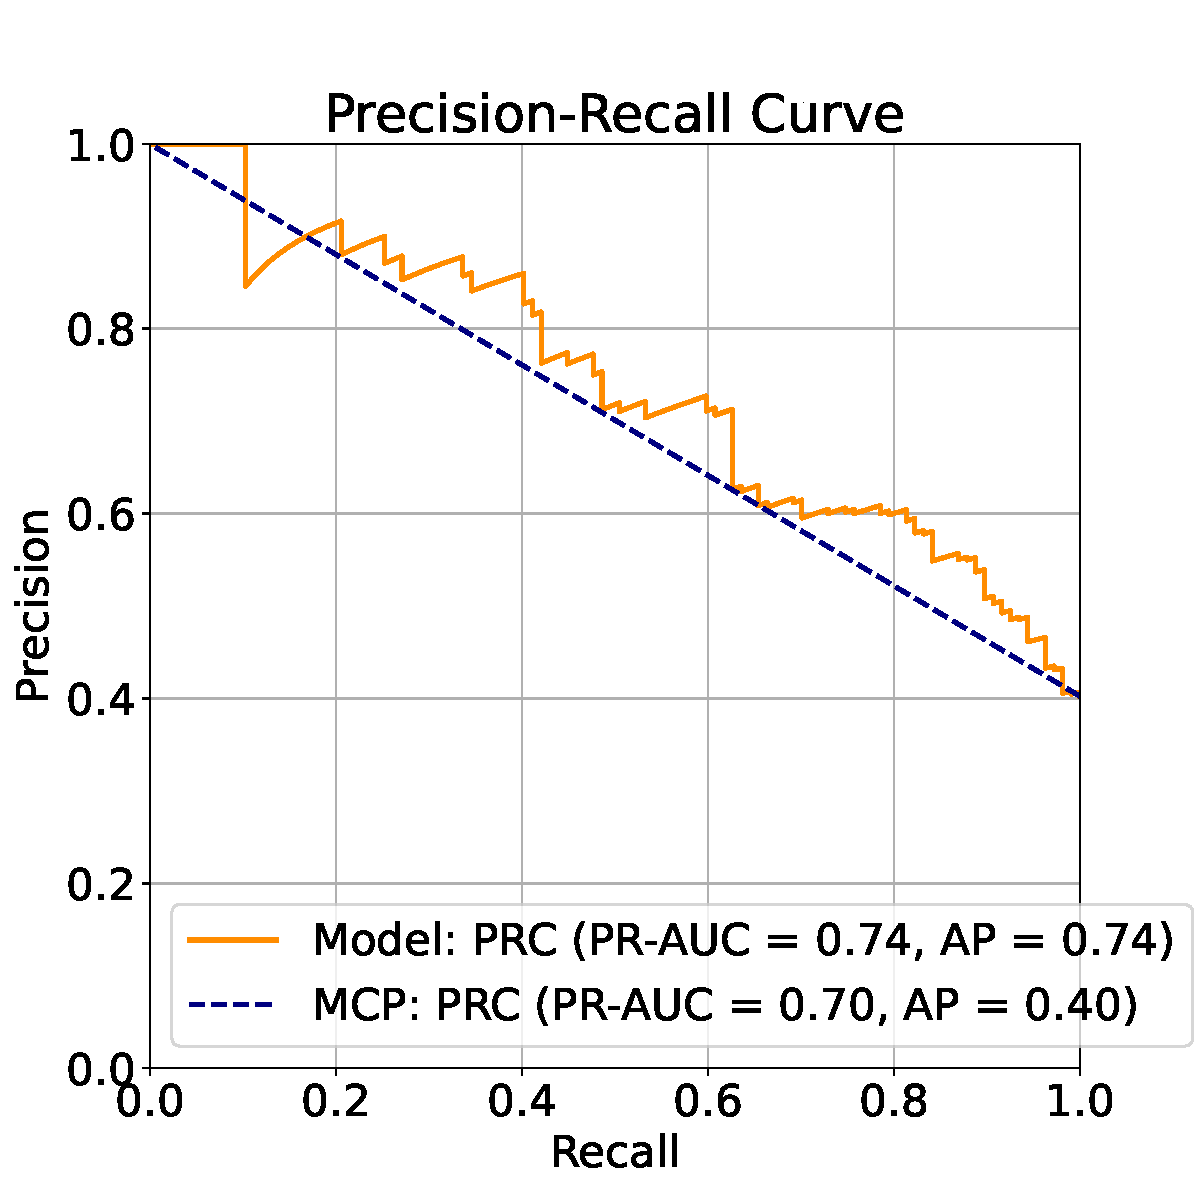
\includegraphics[width=\textwidth / 2]{assets/prc.pdf}
    \caption{Precision-Recall Curve for our LSTM model.}
    \label{fig:prc}
\end{figure}
When comparing PR-AUC across methods, the LSTM model achieved 0.74 (95\% CI: [0.66, 0.82]), comparable to the Twitter Follower Heuristic (0.73, 95\% CI: [0.66, 0.79]) and slightly outperforming the Price Trend Heuristic (0.68, 95\% CI: [0.58, 0.76]). However, the Development Activity Heuristic achieved the highest PR-AUC (0.80, 95\% CI: [0.73, 0.87]), with a confidence interval entirely above the LSTM model’s lower bound. Statistical tests confirmed significant differences between the LSTM model and all heuristics ($p<1 \times 10^{-16}$), with the LSTM outperforming the Price Trend and Twitter Follower Heuristics while the Development Activity Heuristic surpassed the LSTM. For the test, we bootstrapped the PR-AUC one thousand times.
These results suggest that while the LSTM model incorporates multiple signals, its advantage was marginal and did not meet the criterion of noteworthy higher precision, recall, or PR-AUC as evidenced by non-overlapping 95\% confidence intervals. Notably, development activity as a standalone metric outperforms the LSTM. Therefore, we reject our hypothesis. This finding implies that for quick classification of active versus inactive DAOs, relying on development activity alone could be sufficient, offering a more straightforward and equally effective solution compared to the computationally intensive LSTM approach.

In this chapter, we disclosed our results of the LSTM model as well as of all the single input heuristics. We then compared all models and came to the conclusion that the LSTM model outperforms single input heuristics but has a bigger confidence interval. We also compared the LSTM model with the majority class prediction, proving that the LSTM saw patterns in the training data.
In the next chapter, we will discuss why our results have an impact on current DAO research.
